\chapter{多特征卷积神经网络的图像分类方法}


\section{浮游生物图像特点}
自然图像分类主要是将图像中不同物种或不同类别的物体进行相应的归属分类,不同类别或不同类别的物体之间在外观形态上具有较大的差异,因此可根据其外观上形态特点的不同进行区分判断。但是自然图像分类的难点在于物种和种类的多样性,一般的自然图像分类中的种类数目可能在10-100类之间,甚至会有1000类的情况,这为自然图像分类带来巨大难度。在传统的自然图像分类中,通常是对图像提取特定的特征,根据所提取的特征进行相应分类器的训练,使用训练好的分类器对图像进行分类。而细粒度图像分类是在相同基本类别或物种下,对其繁多的子类别进行区分。由于细粒度图像分类属于相同大类的分类,所以各子类别之间的差异很小,这些细微的差异很容易被形状、背景等变化因素影响,导致细粒度图像分类相对困难。因此,细粒度图像分类要求更关注某些具体的细节信息差异,设计更有效的算法实现高准确率分类。对于细粒度图像分类,通常是对某些局部的细节特征信息进行处理,根据这些细微差异进行判断。

浮游生物种群数量庞大,在这种数量级的情况下,不同种类的浮游生物会出现各式各样的形态特点,包括角毛、纹理、扭曲形状等特殊特征。由于浮游生物庞大的种群以及所呈现的不同形态特征,对于该领域的专家和研究学者也很难在短时间内快速和准确地判断浮游生物相对应的种类。尽管浮游生物图像分类问题已经在二十多年前就已经被提出,但是到目前为止仍然没有一个很好的分类方法来解决这个问题,是一个非常具有挑战性的问题。浮游生物图像分类问题的难点主要在两个方面:(1)浮游生物的种类复杂繁多,而且浮游生物不同物种之间可能呈现出多种多样的形态特点,使得一般提取固定特征的方法很难适用于提取这种变化无常的特征;(2)浮游生物图像分类中存在类内差异性和类间相似性。类内差异性表示来自相同类别的浮游生物,在外形特点上呈现非常不相似的情况;而类间相似性表示来自不同类别的浮游生物,在外形特点上却出现及其相似的情况。

\begin{figure}[H]
  \centering%
  \subcaptionbox{} %标题的长度,超过则会换行,如下一个小图。
    {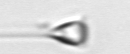
\includegraphics[height=1.6cm]{s1}}%
  \hspace{2em}%
  \subcaptionbox{}
      {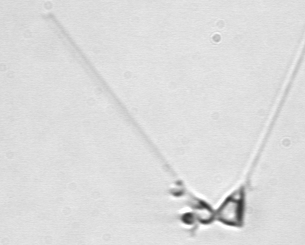
\includegraphics[height=2.5cm]{s2}}
  \hspace{2em}%
  \subcaptionbox{}
      {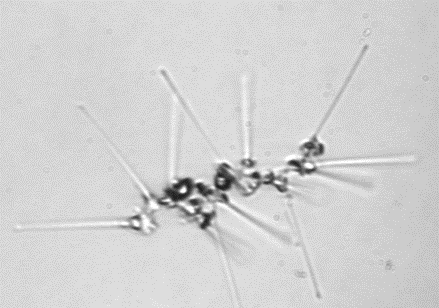
\includegraphics[height=2.5cm]{s3}}
  \caption{来自相同种类中的浮游生物,却表现出不相似的外形,即类内差异性}
\end{figure}

\begin{figure}[H]
  \centering%
  \subcaptionbox{} %标题的长度,超过则会换行,如下一个小图。
    {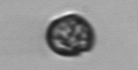
\includegraphics[height=1.8cm]{v1}}%
  \hspace{2em}%
  \subcaptionbox{}
      {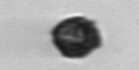
\includegraphics[height=1.8cm]{v2}}
  \hspace{2em}%
  \subcaptionbox{}
      {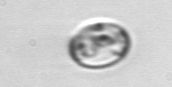
\includegraphics[height=1.8cm]{v3}}
  \caption{来自不同种类的浮游生物,却表现出相似的外形特点,即类间相似性}
\end{figure}


考虑到以上描述的浮游生物图像特点,使浮游生物图像的分类成为处于自然图像分类与细粒度分类之间的一种分类问题,因此依照目前传统的分类方法,即使用人工提取的特征(SIFT,HOG,LBP等)以及多种传统的分类器(NN,SVM,RF,DT等),很难有效地解决浮游生物图像分类问题。因此,在设计与实现浮游生物图像分类方法时,需要考虑浮游生物图像的特点,保证这些问题有效的解决。%但是由于浮游生物图像所存在的特殊性,正常适用于自然图像的特征提取方法,在提取浮游生物图像的特征方面,所取得的效果比较一般;而细粒度图像分类方法根据局部细节信息的判断方法,往往会忽略某些重要的全局特征信息,因此这中方法也不适用于浮游生物图像的分类。

%对于人类来说,首先往往是根据物体的形状进行区分的。但是由于之前我们已经讨论过浮游生物存在类间相似性与类内差异性,所以单纯根据浮游生物的外形形状进行类别的判断是不可靠的。在这种情况下,我们又可以根据浮游生物的纹理特征进行区分,即浮游生物的内部特征。对不同种类的浮游生物而言,其纹理总是不相同。对于同一种浮游生物种类而言,尽管这些浮游生物的形状可能是不相同的,但是纹理总是相似的。所以形状和纹理在浮游生物分类中起着非常重要的作用,为了更准确地对浮游生物图像进行分类,我们应该同时考虑形状特征和纹理特征。因此,在这里我们将原始图像转换为全局特征图像和局部特征图像,分别用来表示形状和纹理特征。随后通过将这些特征图像在卷积神经网络中训练以及混合,提高浮游生物图像的分类准确率。


%%%%%%%%%%%%%%%%%%%%%%%%%%%%%%%%%%%%%%%%%%%%%%%%%%%%%%%%%%%%%%%%%%%%%%%%%%%%%%%%%%%%%%%%%%%%%%%%%%%%%%%%%%%%%%%%%%
\section{多特征卷积神经网络模型}

相比较与传统的人工设计的特征提取和分类器方法,深度学习中的卷积神经网络是基于大量的图像数据以及具有强大学习能力的网络,通过巨大的计算量来获取更抽象和更高维度的信息,目前在图像分类与物体检测方面都取得了非常优异的成果。因此,在这里使用卷积神经网络的学习能力,来解决浮游生物图像分类问题。但是直接使用经典卷积神经网络模型,可能会由于浮游生物图像本身的特点,无法使网络模型发挥良好效果,需要对卷积网络模型进行改进。

\begin{figure}[H]
\centering
\begin{minipage}[b]{0.45\linewidth} 
      \centering 
      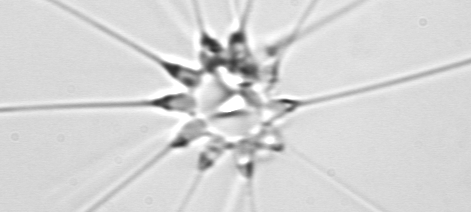
\includegraphics[width=0.75\linewidth]{shape1}
        \centerline{(a) }\medskip
\end{minipage}
  \begin{minipage}[b]{0.45\linewidth}
    \centering
    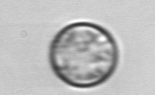
\includegraphics[width=0.65\linewidth]{shape2}
      \centerline{(b) }\medskip
  \end{minipage}
    \begin{minipage}[b]{0.45\linewidth}
    \centering
    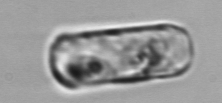
\includegraphics[width=0.75\linewidth]{shape3}
      \centerline{(c) }\medskip
  \end{minipage}
  \begin{minipage}[b]{0.45\linewidth}
    \centering
    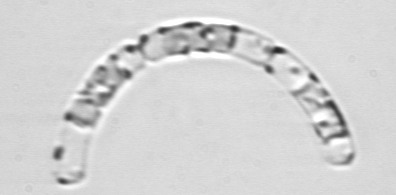
\includegraphics[width=0.75\linewidth]{shape4}
      \centerline{(d) }\medskip
  \end{minipage}
 \caption{不同种类的浮游生物图像}
\label{fig:plankton}
\end{figure}

为了有效地解决浮游生物图像分类问题,首先要对浮游生物图像的特点进行分析。对于人类识别物体,首先从物体的外观获取形状、大小、颜色等信息,通过对这些信息进行处理判断。如图~\ref{fig:plankton}所示,可以看出对于大多数浮游生物而言,不同种类的浮游生物在形状等形态特征方面仍然具有很大的差异,因此人类识别物体优先考虑外部形状,这种方法在浮游生物分类上仍可以使用。

但是如果只单纯从外部形状出发可能会造成很大问题。因为之前讨论过的类间相似性,即不同类别的浮游生物呈现相似的形状,如图~\ref{fig:similarity},如果考虑形状,那么很可能将不同种类的浮游生物归到同一个类别中;同时,由于类内相似性的存在,即相同类别的浮游生物呈现不同的形状,如图~\ref{fig:diff},那么很可能就会将相同类别的浮游生物划分为不同的类别。

\begin{figure}[H]
\centering
\begin{minipage}[]{0.42\linewidth} 
      \centering 
      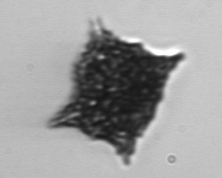
\includegraphics[height=3.2cm]{similarity1}
        \centerline{(a) }\medskip
\end{minipage}
  \begin{minipage}[]{0.42\linewidth}
    \centering
    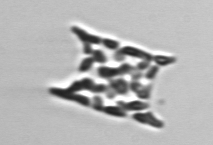
\includegraphics[height=3.1cm]{similarity2}
      \centerline{(b) }\medskip
  \end{minipage}
 \caption{两个不同种类的浮游生物图像,形状相似}
\label{fig:similarity}
\end{figure}

\begin{figure}[H]
\centering
\begin{minipage}[]{0.42\linewidth} 
      \centering 
      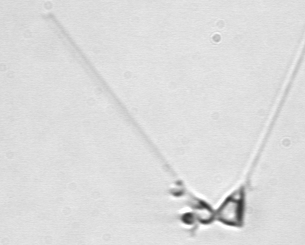
\includegraphics[height=3.2cm]{diff1}
        \centerline{(a) }\medskip
\end{minipage}
  \begin{minipage}[]{0.42\linewidth}
    \centering
    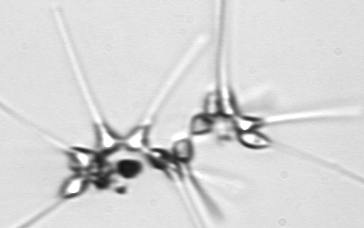
\includegraphics[height=3.1cm]{diff2}
      \centerline{(b) }\medskip
  \end{minipage}
 \caption{两个相同种类的浮游生物图像,形状不同}
\label{fig:diff}
\end{figure}

通过对浮游生物图像的不断研究,随后又发现了浮游生物内部的纹理具有很强的区分性。对于不同的浮游生物,内部纹理往往是不同的,如图~\ref{fig:texture1};而对于相同的浮游生物而言,纹理基本是相同的,如图~\ref{fig:texture2}。因此, 对于实现浮游生物图像分类,除了依靠形状信息外,纹理信息也是区分浮游生物的另一个重要特征。

\begin{figure}[H]
\centering
\begin{minipage}[]{0.45\linewidth} 
      \centering 
      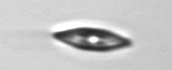
\includegraphics[height=2cm]{1}
        \centerline{(a) }\medskip
\end{minipage}
  \begin{minipage}[]{0.45\linewidth}
    \centering
    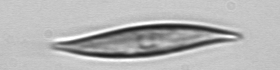
\includegraphics[height=1.7cm]{2}
      \centerline{(b) }\medskip
  \end{minipage}
 \caption{两个不同种类的浮游生物图像,纹理不同}
\label{fig:texture1}
\end{figure}

\begin{figure}[H]
\centering
\begin{minipage}[]{0.3\linewidth} 
      \centering 
      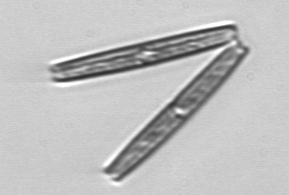
\includegraphics[height=2.5cm]{3}
        \centerline{(a) }\medskip
\end{minipage}
  \begin{minipage}[]{0.3\linewidth}
    \centering
    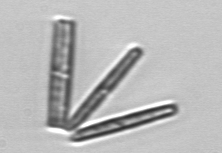
\includegraphics[height=2.5cm]{4}
      \centerline{(b) }\medskip
  \end{minipage}
  \begin{minipage}[]{0.3\linewidth}
    \centering
    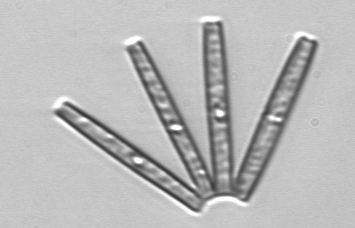
\includegraphics[height=2.5cm]{5}
      \centerline{(c) }\medskip
  \end{minipage}
  \caption{三个相同种类的浮游生物图像,纹理相同}
\label{fig:texture2}
\end{figure}

考虑到浮游生物图像所存在的类间相似性和类内差异性问题,可以结合形状信息和纹理信息,对浮游生物图像进行区分,但是在提取转换形状和纹理时,可能会造成浮游生物图像中部分重要信息的缺失,并且形状信息和纹理信息的侧重点不同,很难完美地进行结合,所以仍然需要对原始图像进行处理,提取所有信息。综合考虑以上因素,本论文提出了一种基于多特征卷积神经网络的浮游生物图像分类方法。

在生物形态学的角度,浮游生物图像中的形状信息和纹理信息是分析和处理浮游生物图像的关键信息;在计算机视觉的角度,可以将浮游生物图像的所有信息、形状信息和纹理信息转换为图像的原始特征、全局特征和局部特征。因此,在本网络模型中使用了三种不同的特征提取方法来描述浮游生物图像的特征,即原始特征、全局特征和局部特征,分别对应了图像中浮游生物的所有信息、形状信息和纹理信息。通过将这三种特征图像在模型中三个独立的卷积神经子网络中分别训练,不同子网络之间相互独立,使这些子网络只注重全部信息、形状信息和纹理信息这些具体特征的提取转换,而不用注重其他信息。在模型的最后部分是全连接层,通过对全连接层的交叉处理,保证不同特征的充分融合,对最终结果进行决策输出。

本论文所提出的多特征卷积神经网络模型结构如图~\ref{fig:architecture}所示。本网络模型是由三个卷积神经子网络组成,将这些子网络从左至右分别标记为网络A,网络B和网络C,从训练时间、网络大小以及网络性能等方面考虑,选择AlexNet作为基础子网络,不过不包括全连接层部分。本网络模型的1-5层为卷积层,6-8层为全连接层。

\begin{figure}[H] % use float package if you want it here
  \centering
  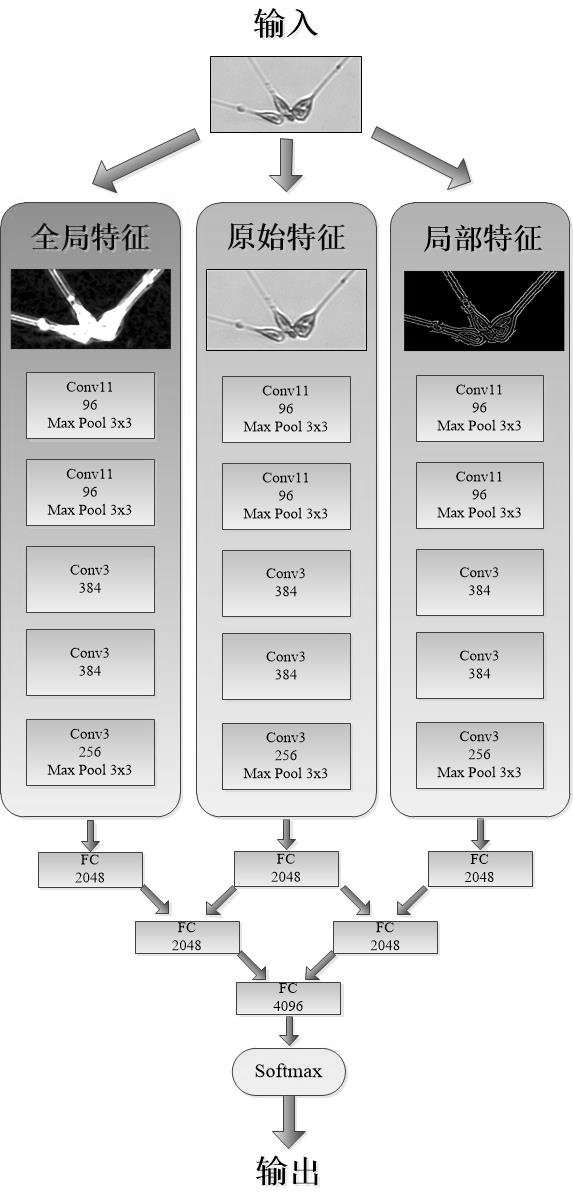
\includegraphics[height=17cm]{architecture}
  \caption{浮游生物图像分类的多特征卷积神经网络模型}
  \label{fig:architecture}
\end{figure}

如图~\ref{fig:architecture}所示,子网络A的第一个包含conv的方框表示卷积层,conv11表示卷积核的大小为11x11,96表示卷积核数目为96,Max pooling表示使用最大值池化,池化范围为3x3的像素块。同理,子网络A的最后一个包含conv的方框也表示卷积层,conv3表示卷积核的大小为3x3,384表示卷积核数目为384,Max pooling表示使用最大值池化,池化范围为3x3的像素块。第6层以后包含FC的方框表示全连接层,其中2048表示全连接层中神经元的个数。子网络A用来训练全局特征图像,子网络B用来训练原始图像,子网络C用来训练局部特征图像。其中,用来训练子网络A和C的全局特征图像和局部特征图像,输入图像在输入层经过数字图像处理和计算机视觉方法转换得到的。由于原始图像和全局特征图像以及局部特征图像之间有相同的尺寸,因此保证了各个网络的特征映射之间具有融合的可能性。在卷积层之后,本模型使用了倒金字塔形状的全连接结构,称之为交叉全连接层。考虑到在全局特征和局部特征之间具有巨大的差异,必须采取有效特殊的全连接结构实现特征融合,消除特征间的间隔。这里的交叉全连接层将两个子网络卷积之后的结果进行两两结合(全局特征与原始特征,原始特征与局部特征),最后将剩余两个结果进行融合,即通过原始图像所得到的内积作为连接局部特征和全局特征的桥梁。尽管该模型有三个输入数据,但是在网络处理和融合后只有一个输出,因此在训练过程的反向传播中,三个子网络共享同一个标签以及损失函数,保证了网络能够得到正常的训练。


%%%%%%%%%%%%%%%%%%%%%%%%%%%%%%%%%%%%%%%%%%%%%%%%%%%%%%%%%%%%%%%%%%%%%%%%%%%%%%%%%%%%%%%%%%%%%%%%%%%%%%%%%%%%%%%%%%%
\section{特征提取和特征融合}

\subsection{原始特征}
对于原始特征,我们需要采取基本的预处理:镜像映射、调整尺度、随机裁剪和减均值处理。图~\ref{fig:origin:a}表示输入到卷积神经网络模型的原始图像,图~\ref{fig:origin:b}表示原始图像经过调整尺度后的形式,蓝色方框代表随机裁剪后的区域。

\begin{figure}[H]
  \centering%
  \subcaptionbox{\label{fig:origin:a}} %标题的长度,超过则会换行,如下一个小图。
    {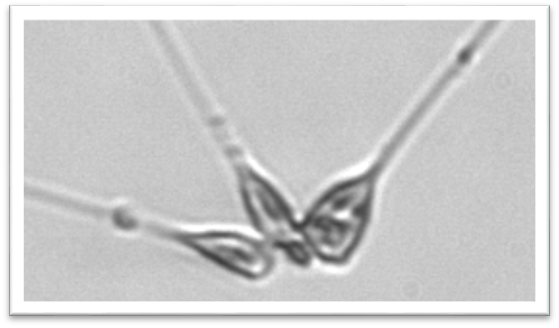
\includegraphics[height=3cm]{o}}%
  \hspace{4em}%
  \subcaptionbox{\label{fig:origin:b}}
      {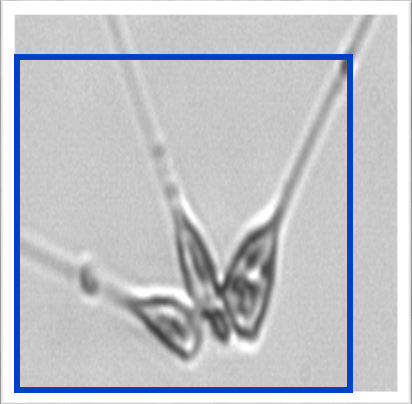
\includegraphics[height=3.5cm]{oa}}
  \caption{原始图像和经过预处理后的结果}
  \label{fig:origin}
\end{figure}

对于原始特征的预处理方法:
\begin{itemize}
\item 镜像映射:深度学习由于样本数据、网络模型以及训练方法的限制,经常会造成网络的过拟合。而最简单,也是最常用的方法是通过扩大数据集图像数量的方法来降低过拟合。镜像映射就是一种数据增强方法,通过在垂直方向上的映射,拓展样本数据的多样性。
\item 调整尺度:由于数据集中的图像大小经常不一致,而卷积神经网络对所有图像进行统一处理,因此在输入的时候,需要将图像进行尺度的调整。这里将所有图像的大小调整为256x256的形式,保证了所有输入图像尺度的统一,以及正常的训练。
\item 随机裁剪:图像中有许多信息是冗余的,而通过对输入图像的随机裁剪可以降低数据的维度,减少网络的计算量。另一方面,经过随机裁剪后的图像,一定程度增加了数据的随机性,可以降低过拟合现象。经过剪裁后图像的大小为224x224。
\item 减均值处理:根据所有输入图像计算出相应的均值图像,将每张图像的像素值进行减均值处理,是一种归一化方法,可以保证网络的有效训练,可以加快训练速度。另外,经过减均值处理,可以一定程度地提升准确率。
\end{itemize}



\subsection{全局特征}

由于网络模型中的全局特征表示了浮游生物的形状信息,而浮游生物的角毛和轮廓等形态特点都被视为是重要的形状信息\cite{zheng2014automatic},这些形态特点也是用来区分浮游生物种类的重要依据。所以,根据形状进行浮游生物类别的判断,是最直观也是最常用的方法。

但是想要提取出完整的浮游生物形状却不是容易的事情。由于浮游生物的形状较为复杂,细长的角毛、透明的细胞外膜、内部明显的细胞等因素,造成了浮游生物在外观形状上呈现多样化趋势;同时,因为浮游生物的角毛或细胞膜都为透明的,与背景十分相似,需要仔细观察才能够辨别出来。基于以上问题,使得传统的轮廓提取和图像分割的方法在提取浮游生物的形状信息时,都没有取得很好的效果。

因为形状信息主要注重浮游生物的外部轮廓,而不必关注内部纹理与图像背景。因此,如果能够突出浮游生物的形状轮廓,使其与背景产生强烈反差,即可有效提取出形状信息。在这里,本论文提出了一种图像处理的方法来解决这个问题,使图像中浮游生物的形状相比较于其它特征显得更明显与突出。
\begin{enumerate}
\item 首先,使用双边滤波器\cite{tomasi1998bilateral}消除浮游生物图像中的部分噪声,使图像中的浮游生物形状更加平滑。
\item 其次,使用基于Sobel算子优化的Scharr算子\cite{scharr2000optimal}将原始浮游生物图像转换为同时包含形状与纹理的图片形式。
\item 随后,为了使全局形状特征更加明显突出,由于浮游生物整体亮度较大,而背景颜色较深,因此使用对比度增强方法,使形状更加明显,移除内部特征。
\item 最后,经过对比度增强后的图像,可认为是充分表达形状信息的全局特征图像。
\end{enumerate}

\begin{figure}[H]
\centering
\begin{minipage}[]{0.3\linewidth} 
      \centering 
      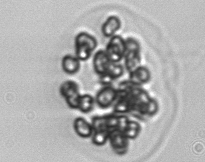
\includegraphics[height=2.5cm]{g1}
        \centerline{(a) }\medskip
\end{minipage}
  \begin{minipage}[]{0.3\linewidth}
    \centering
    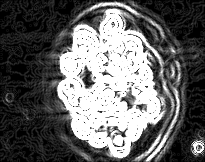
\includegraphics[height=2.5cm]{g2}
      \centerline{(b) }\medskip
  \end{minipage}
  \begin{minipage}[]{0.3\linewidth}
    \centering
    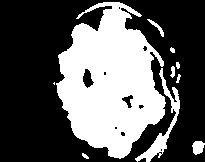
\includegraphics[height=2.5cm]{g3}
      \centerline{(c) }\medskip
  \end{minipage}
\begin{minipage}[]{0.3\linewidth} 
      \centering 
      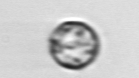
\includegraphics[height=2.2cm]{g4}
        \centerline{(d) }\medskip
\end{minipage}
  \begin{minipage}[]{0.3\linewidth}
    \centering
    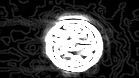
\includegraphics[height=2.2cm]{g5}
      \centerline{(e) }\medskip
  \end{minipage}
  \begin{minipage}[]{0.3\linewidth}
    \centering
    
\includegraphics[height=2.2cm]{g6}
      \centerline{(f) }\medskip
  \end{minipage}
  \caption{原始浮游生物图像,使用图像处理方法和图像分割方法得到的结果}
\label{fig:shape}
\end{figure}

图4-10(a)表示原始浮游生物图像,图4-10(b)表示经过本论文方法提取的全局特征图像,图4-10(c)表示使用图像分割技术grabcut\cite{rother2004grabcut}取得的全局特征图像。仅从外观上而言,图4-10(b)外观形状更明显,而图4-10(c)有部分形状信息缺失。图4-10(e)和图4-10(f)表示当grabcut方法能够有效地转换全局特征图像时,本论文方法也可以取得相应的结果。另外,将这些全局特征图像在AlexNet中进行实验,实验结果也表明了使用本论文的图像处理方法转换的全局特征图像所训练的网络,最终的分类准确率优于其他方法的结果。

\subsection{局部特征}

因为只根据形状信息区分浮游生物图像,结果往往是不可靠的。为了更有效的对浮游生物图像分类,需要另一个特征对形状信息进行补充。而由上述介绍可知,纹理信息相对于形状信息,是浮游生物另外一个非常重要的特征。相同种类的浮游生物,内部纹理基本相同;不同种类的浮游生物,内部纹理基本不相似。因此,可以使用纹理信息作为区分浮游生物种类的另外一个重要特征。

Canny算法\cite{canny1986computational}是一个多阶层的边缘算法,可以用来检测图像中大范围的边缘。Canny算法的目标在于检测图像中的最优边缘,即尽可能多地标识出图像中的实际边缘。这里将内部纹理信息理解为局部特征,使用Canny算法对内部特征进行提取转换。Canny算法的步骤可归纳为:
\begin{enumerate}
\item 降噪:通过将高斯平滑模板对原始图像进行卷积运算,得到有轻微模糊的图像。
\item 寻找图像中的亮度梯度:图像中的边缘可能会指向不同方向,这里使用水平方向、垂直方向以及对角线方向的4个掩膜对原始图像进行卷积运算。随后标注出各个像素点中的最大像素值和所生成的边缘方向,即可得到图像中像素点的亮度梯度图和亮度梯度方向。
\item 在图像中跟踪边缘:使用滞后阈值(高阈值和低阈值)对图像中的重要边缘进行跟踪标记,避免将噪声像素标记为边缘。
\end{enumerate}

通过对Canny算法中可调整参数(高斯滤波器的大小和阈值的设置)的修改,使Canny算法有效地跟踪标记出浮游生物的内部纹理信息,提取出浮游生物的纹理信息。图~\ref{fig:texture}表示原始图像和经过Canny算法转换后的局部特征图像。图4-11(a)和图4-11(c)从外观形状上非常相似,但是经过Canny算法提取局部特征之后,从图4-11(c)和图4-11(d)可以看出其内部纹理不相同,根据这点可对浮游生物图像进行区分。

\begin{figure}[H]
\centering
\begin{minipage}[b]{0.45\linewidth} 
      \centering 
      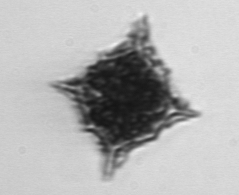
\includegraphics[width=0.75\linewidth]{l1}
        \centerline{(a) }\medskip
\end{minipage}
  \begin{minipage}[b]{0.45\linewidth}
    \centering
    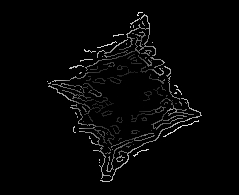
\includegraphics[width=0.75\linewidth]{l2}
      \centerline{(b) }\medskip
  \end{minipage}
    \begin{minipage}[b]{0.45\linewidth}
    \centering
    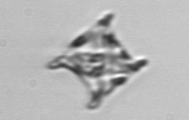
\includegraphics[width=0.75\linewidth]{l3}
      \centerline{(c) }\medskip
  \end{minipage}
  \begin{minipage}[b]{0.45\linewidth}
    \centering
    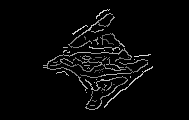
\includegraphics[width=0.75\linewidth]{l4}
      \centerline{(d) }\medskip
  \end{minipage}
 \caption{不同种类的浮游生物图像以及经过Canny算法转换的局部特征图像}
\label{fig:texture}
\end{figure}


%%%%%%%%%%%%%%%%%%%%%%%%%%%%%%%%%%%%%%%%%%%%%%%%%%%%%%%%%%%%%%%%%%%%%%%%%%%%%%%%
\subsection{交叉全连接层}

传统的网络融合方法主要是在全连接层计算后,直接对矢量相连进行融合。但是由于全局特征图像与局部特征图像是针对不同的视觉特点所提取的,那么在卷积神经网络训练时,最终所关注的重点信息将会有极大差别,如果直接融合可能反而会造成准确率的下降,因此需要一个更好的特征融合方式来提升分类结果。



如图4-12(a)表示普通的全连接融合,即只在最后一层进行矢量连接输出。但是由于在网络模型中,之前的子网络训练的特征具有较大差异,直接融合反而可能不会提升效果。原始图像中不仅具有全局特征,也包括局部特征。如果以原始特征为中介,进行融合以及继续训练,那么将能够更好地消除不同特征之间的间隙,实现特征的融合。因此本论文提出了以下的倒金字塔形式的全连接方式,即交叉全连接层,如图4-12(b)所示。交叉全连接层通过将不同特征进行两两结合,实现特征的融合以及重训练。

\begin{figure}[H]
\centering
\begin{minipage}[]{0.8\linewidth} 
      \centering 
      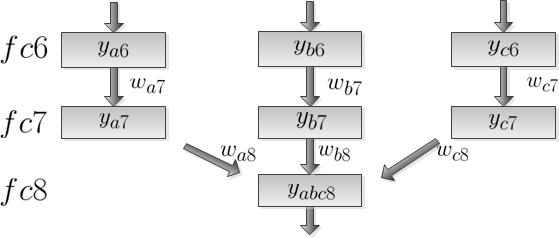
\includegraphics[height=4cm]{f1}
        \centerline{(a) }\medskip
\end{minipage}
  \begin{minipage}[]{0.8\linewidth}
    \centering
    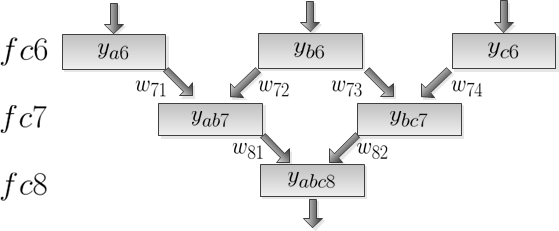
\includegraphics[height=4cm]{f2}
      \centerline{(b) }\medskip
  \end{minipage}
 \caption{普通全连接层融合以及交叉全连接层}
%\label{fig:diff}
\end{figure}


FC6表示第六层为全连接层,同理,FC7和FC8同为全连接层。与之前所讨论的全连接层计算方式不同,从第6层到第7层的全连接训练的前向过程可以被归纳以下形式:
\begin{align}
y_{ab7m}=f(\sum_{i}^{2048} w_{71im}  y_{a6i} + \sum_{j}^{2048} w_{72jm}  y_{b6j} + b_{ab7}) \\
y_{bc7n}=f(\sum_{j}^{2048} w_{73jn}  y_{b6j} + \sum_{k}^{2048} w_{74kn}  y_{c6k} + b_{bc7}) 
\end{align}
$y_{ab7m}$表示第7层全连接层的左边层中第$m$个神经元的输出,$y_{bc7n}$表示第7层全连接层的右边层中的第$n$个神经元的输出。$w_{71im}$是第6层的第$i$个神经元到第7层的第$m$个神经元之间所对应的权值,$y_{a6i}$是子网络A中第6层的第$i$个神经元,$y_{b6j}$是子网络B中第6层的第$j$个神经元,$y_{c6k}$是子网络C中第$k$个神经元,$b_{ab7}$是第7层左边的偏置项,$b_{bc7}$是第7层右边的偏置项。相似的,$y_{abc8o}$也可以推导出。
\begin{equation}
y_{abc8o}=f(\sum_{m}^{4096} w_{81mo}  y_{ab7m} + \sum_{n}^{4096} w_{82no}  y_{bc7n} + b_{abc8})
\end{equation}

在反向传播时,误差传播相应的规则也必须遵从之前所提出的金字塔结构。特别地,在子网络B中,第6层的误差导数可以表示为如下形式:
\begin{equation}
\delta_{b6j}=f'(x_{b6j}) (\delta_{ab7m}  w_{72mj} + \delta_{bc7n}  w_{73nj})
\end{equation}
其中$\delta_{b6j}$是子网络B中第6层的第$j$个神经元的误差,$f'(x)$是激活函数的导数,请注意,只有子网络B会接收到从最后一层所传回的所有反向误差,而网络A和网络B将只接受从第8层传回的部分误差。

%%%%%%%%%%%%%%%%%%%%%%%%%%%%%%%%%%%%%%%%%%%%%%%%%%%%%%%%%%%%%%%%%%%%%
\section{具体步骤}

基于多特征融合卷积神经网络的浮游生物图像分类方法包括下列的具体步骤:
\begin{enumerate}
\item 采集清晰的浮游生物图像,构建大规模多类别的浮游生物图像数据集。该数据集中的浮游生物图像即为输入图像,在输入层对浮游生物输入图像进行预处理;

\item 通过对输入图像进行镜像映射、尺度调整、随机裁剪等预处理,得到原始特征图像


\item 通过对输入图像进行相应的数字图像处理,提取浮游生物的形状信息,得到全局特征图像:
\begin{enumerate}
\item 利用双边滤波法消除图像中的噪声,平滑图像中浮游生物的外部形状;
\item 利用Scharr算法对滤波后图像进行转换,得到中间结果图;
\item 使用增强对比度处理中间图,突出浮游生物的全局特征,忽略浮游生物的局部特征,得到的结果即为全局特征图像;
\end{enumerate}

\item 通过对输入图像使用计算机视觉中的Canny边缘检测算法,提取浮游生物内部的纹理信息,即浮游生物的局部特征,得到局部特征图像;

\item 将步骤2、步骤3及步骤4得到的原始特征图像、全局特征图像及局部特征图像输入到该多特征融合卷积神经网络模型中进行训练,最终得到优化后的多特征融合卷积神经网络模型:
\begin{enumerate}
\item 首先设置网络初始状态信息,包括迭代次数、学习率及初始化方式;
\item 对该多特征融合卷积神经网络模型进行前向和后向传播,使该多特征融合卷积神经网络模型以损失函数值为基础,根据权值梯度下降方向,对权值等参数进行更新和学习;
\item 随着不断迭代,损失函数值逐步下降,相应的准确率稳步上升;
\item 判断是否达到设置的迭代次数,如果是,则训练完毕,得到最终的多特征融合卷积神经网络模型;否则,继续跳转执行步骤6(b)继续训练;
\end{enumerate}

%\item 构建基于原始特征、全局特征及局部特征的多特征融合卷积神经网络模型,该多特征融合卷积神经网络包括三个相互独立的子网络,每个子网络分别训练原始特征图像、全局特征图像及局部特征图像,其中,该多特征融合卷积神经网络的1-5层为卷积层,6到8层为交叉全连接层;

\item 将待分类的浮游生物图像输入到最终的多特征融合卷积神经网络模型中,即可实现有效的浮游生物图像分类。 

\end{enumerate}

%进一步地,根据实际情况和需求,混合模型中的基础子网络可以使用AlexNet、GoogLeNet或者VGGNet中的任意一种基础卷积神经网络,混合模型最终的准确率根据所选择基础子网络的不同,会逐步提升,而相应地,模型训练时间代价也会逐步增长。

%%%%%%%%%%%%%%%%%%%%%%%%%%%%%%%%%%%%%%%%%%%%%%%%%%%%%%%%%%%%%%%%%%
\section{本章小结}
本章节主要介绍了本论文针对浮游生物图像分类问题,提出了基于多特征卷积神经网络结构模型具体的实现方法。由于浮游生物的种类庞大繁多,并且浮游生物存在类间相似性和类内差异性,使得普通的特征提取方法或机器学习都不能有效解决浮游生物图像分类问题。这里考虑到形状信息和纹理信息是辨别浮游生物种类重要的依据,另外原始图像也包含了重要的信息,因此将这三个特征图像都放在网络中进行训练与特征融合。多特征卷积神经网络模型是由三个卷积子网络组成,使用交叉全连接层实现特征的决策融合,是一个适用于浮游生物图像分类的深层卷积神经网络模型。








